% ============================================================
% Filtros Pasa-bajas (Low-Pass)
% ============================================================
\section{Filtros Pasa-bajas (Low-Pass)}

\subsection{Butterworth}

\begin{figure}[H]
	\centering
	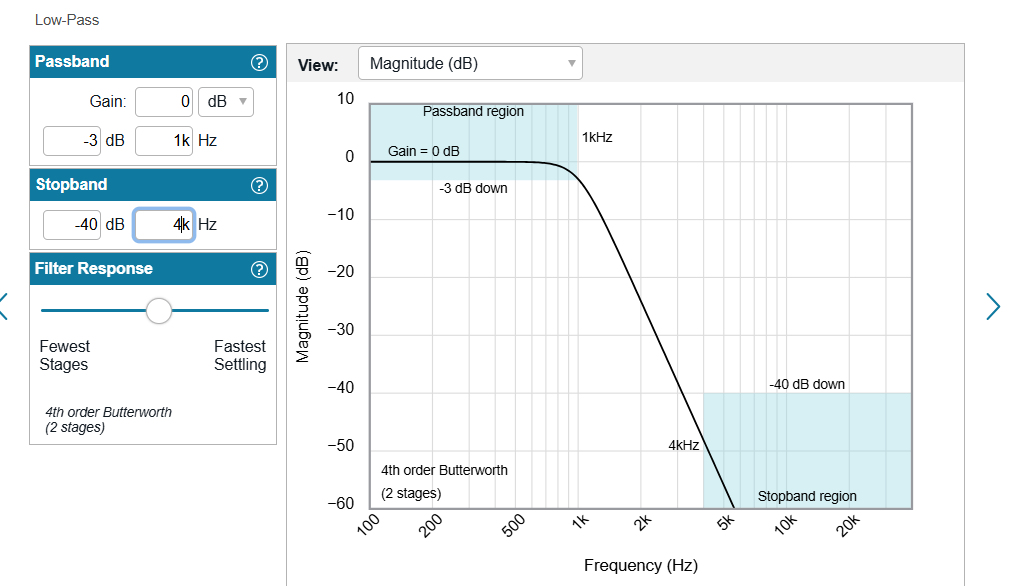
\includegraphics[width=0.9\textwidth]{img/lp_butterworth_respuesta.png}
\end{figure}

\begin{table}[H]
	\centering
	\renewcommand{\arraystretch}{1.2}
	\begin{tabular}{|l|l|}
		\hline
		\textbf{Parámetro} & \textbf{Nuestro diseño} \\
		\hline
		Tipo & Pasa-bajas \\
		Respuesta & Butterworth \\
		Orden & 4.\textsuperscript{o} \\
		Etapas & 2 \\
		Ganancia & 0\,dB \\
		Atenuación banda pasante & $-3$\,dB \\
		Frecuencia banda pasante & 1\,kHz \\
		Atenuación banda rechazo & $-40$\,dB \\
		Frecuencia banda rechazo & 4\,kHz \\
		\hline
	\end{tabular}
\end{table}

\textbf{STAGES}

\begin{figure}[H]
	\centering
	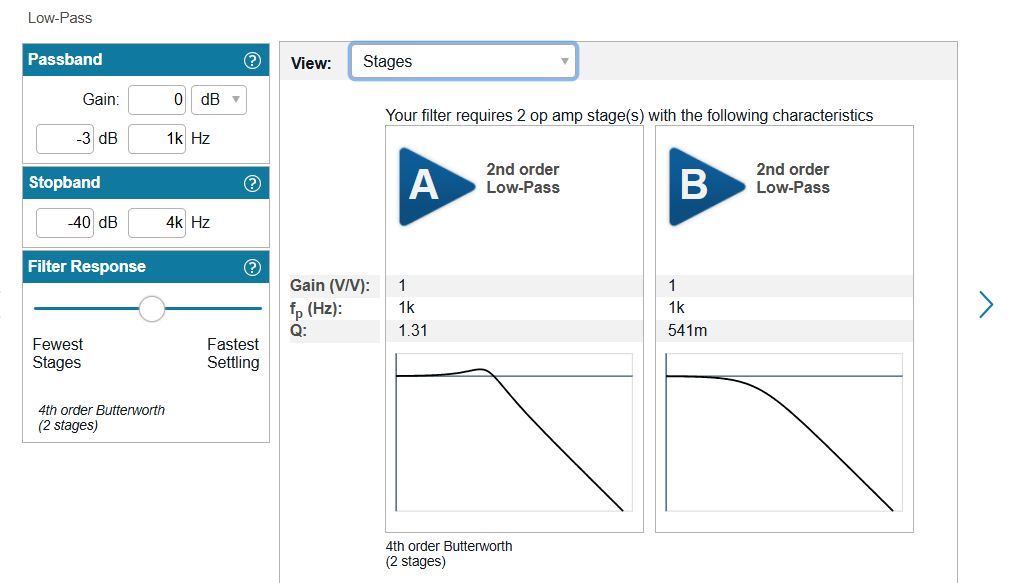
\includegraphics[width=0.9\textwidth]{img/lp_butterworth_etapas.png}
\end{figure}

\subsubsection{¿Qué es Q?}

No quiero que solamente copies ese número sin saber qué significa.

El factor de calidad $Q$ describe qué tan ``selectiva'' o resonante es una etapa de segundo orden.

En un Butterworth de cuarto orden, las dos etapas no tienen necesariamente el mismo $Q$.

Aproximadamente tendremos:
\begin{equation*}
	Q_1 \approx 0.541 \qquad Q_2 \approx 1.307
\end{equation*}

Esto es normal.

\textbf{CIRCUIT}

\begin{figure}[H]
	\centering
	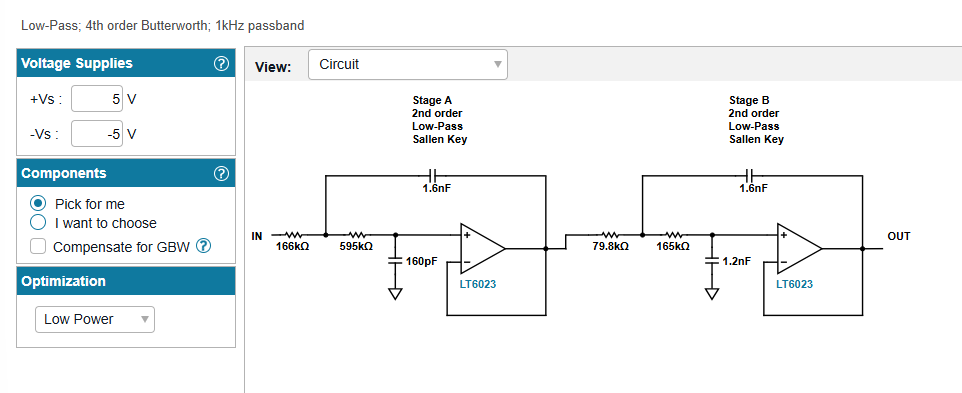
\includegraphics[width=\textwidth]{img/lp_butterworth_circuito.png}
\end{figure}

% ------------------------------------------------------------
\subsection{Chebyshev}

\begin{figure}[H]
	\centering
	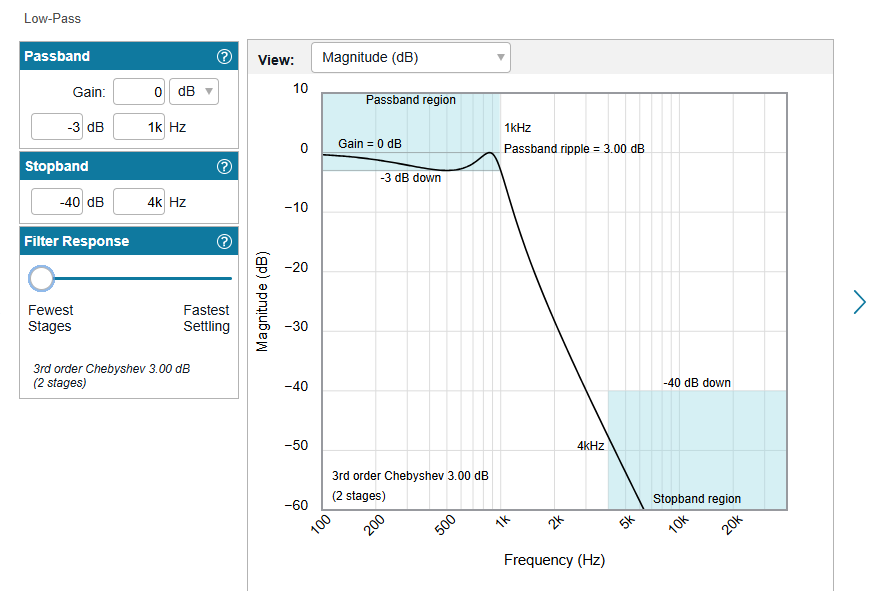
\includegraphics[width=0.9\textwidth]{img/lp_chebyshev_respuesta.png}
\end{figure}

\textbf{Stages}

\begin{figure}[H]
	\centering
	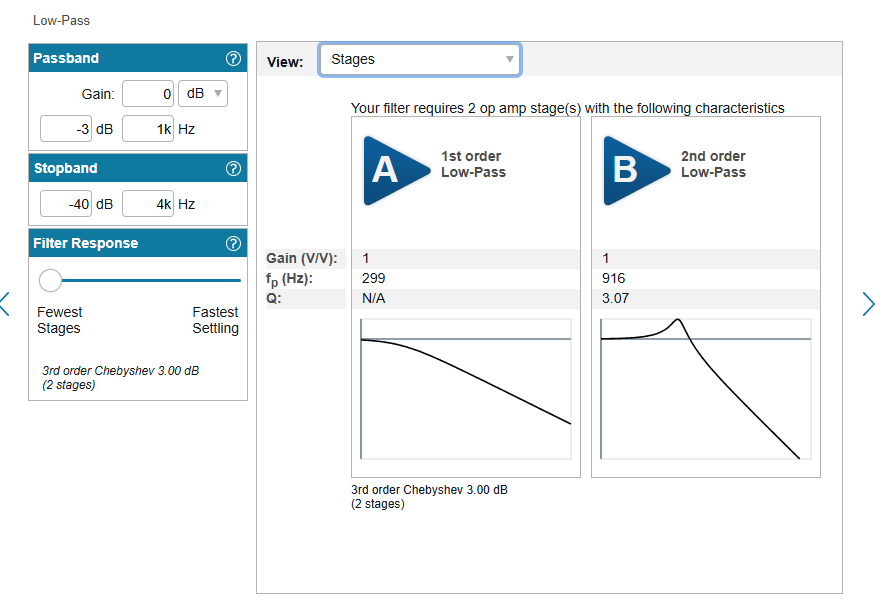
\includegraphics[width=0.9\textwidth]{img/lp_chebyshev_etapas.png}
\end{figure}

\textbf{Circuito}

\begin{figure}[H]
	\centering
	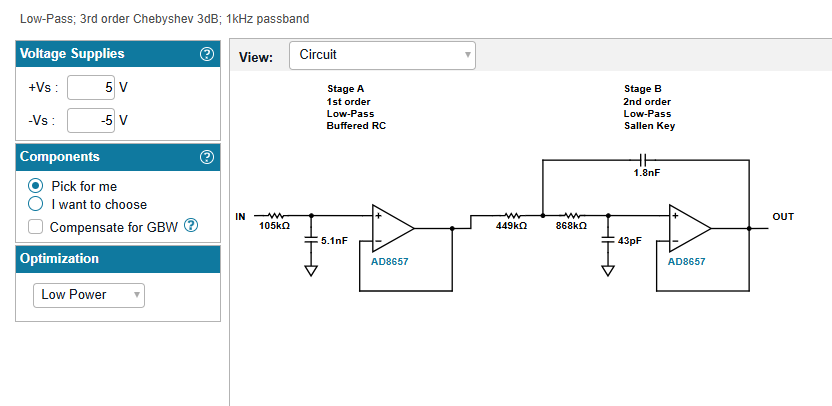
\includegraphics[width=\textwidth]{img/lp_chebyshev_circuito.png}
\end{figure}

% ------------------------------------------------------------
\subsection{Bessel}

\begin{figure}[H]
	\centering
	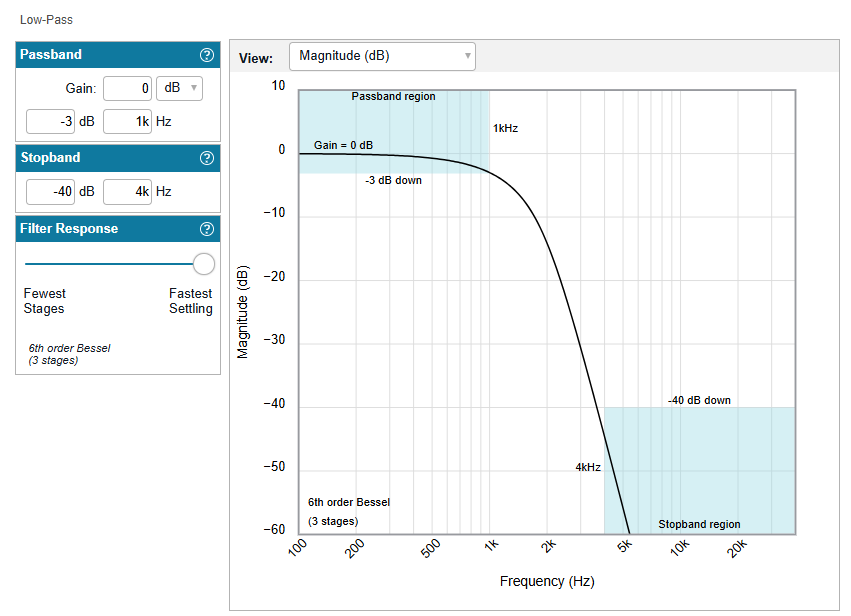
\includegraphics[width=0.9\textwidth]{img/lp_bessel_respuesta.png}
\end{figure}

\textbf{Stages}

\begin{figure}[H]
	\centering
	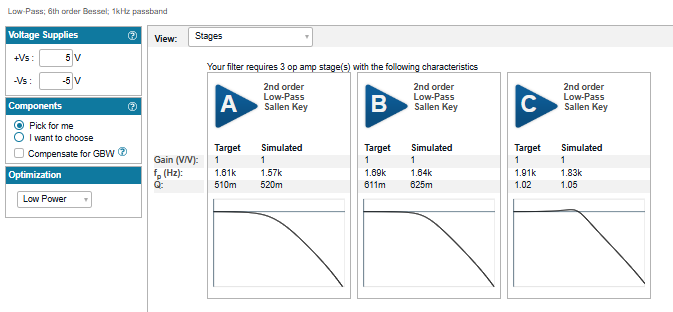
\includegraphics[width=0.9\textwidth]{img/lp_bessel_etapas.png}
\end{figure}

\textbf{Circuito}

\begin{figure}[H]
	\centering
	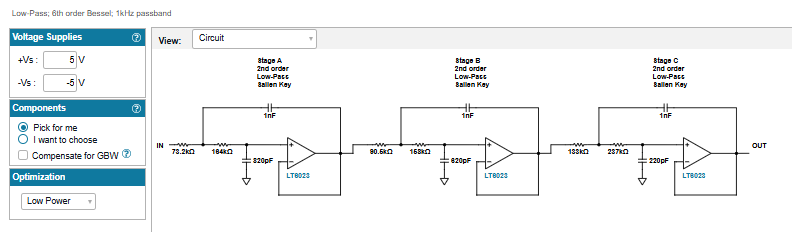
\includegraphics[width=\textwidth]{img/lp_bessel_circuito.png}
\end{figure}
